\documentstyle[doublespace]{article}
%\documentstyle[epsfig,preprint]{pubform}
%\documentclass[epsfig]{acm_proc_article-sp}

\title{A Stream Compiler for Communciation-Exposed Architectures}

\author{Michael Gordon, Bill Thies, Michal Karczmarek, Jeremy Wong,
        Henry Hoffmann, David Maze and Saman Amarasinghe\\
	MIT Laboratory for Computer Science\\
	Cambridge, MA  02139\\
	\sffamily{\{mgordon, thies, karczma, jnwong, hank, dmaze, saman\}@lcs.mit.edu}}
%\date{\today}

% \sloppy lets Latex be a little less anal about interword spacing.  It is
% one way to eliminate those annoying Overfull hbox warnings.
% Another way is to surround each offending paragraph with
% \begin{sloppypar} ... \end{sloppypar}

\sloppy

% See page 90 of the Latex book for info about vertical spacing probs.

\begin{document}
%\toappear{\centerline{\Large\bf MIT LCS Technical Memo,}
%          \centerline{\Large\bf MIT-LCS-TM-6XX,}
%          \centerline{\Large\bf November, 2001.}}

\maketitle

\begin{abstract}
Due to the high data rates involved in audio, video, and signal
processing applications, it is imperative to compress the data to
decrease the amount of storage used.  Unfortunately, this implies that
any program operating on the data needs to be wrapped by a
decompression and re-compression stage.  Re-compression can incur
significant computational overhead, while decompression swamps the
application with the original volume of data.

In this paper, we present a program transformation that greatly
accelerates the processing of compressible data.  Given a program that
operates on uncompressed data, we output an equivalent program that
operates directly on the compressed format.  Our transformation
applies to stream programs, a restricted but useful class of
applications with regular communication and computation patterns.  Our
formulation is based on LZ77, a lossless compression algorithm
utilized by ZIP, and immediately applies to simpler formats such as
Apple Animation, Microsoft RLE, and Targa.

We implemented a simple subset of our techniques in the StreamIt
compiler, which emits executable plugins for two popular video editing
tools: MEncoder and Blender.  For common operations such as color
adjustment and video compositing, computing directly on compressed
data offers a speedup roughly proportional to the overall compression
ratio.  For our benchmark suite of 12 videos in Apple Animation
format, speedups range from 1.1x to 471x, with a median of 15x.

\end{abstract}

%%% Upward of fifty percent of the code that runs the DSP(s) in a modern
%% cell phone is coded in assembly with the rest written in C. Hand
%% optimized assembly code typically makes the best use of the available
%% resources such as power, specialized coprocessors, and specialized
%% instructions.  The problem with assembly code is that the same
%% algorithm must be mapped time and time again whenever a new chip comes
%% out. The life cycle of a typical DSP is much shorter than the life
%% cycle of a general purpose microprocessor -- each new generation is
%% separated by months rather than years.
 
%% Therefore frequently reimplementing algorithms by hand is a costly,
%% arduous process that increases cost and slows the pace of
%% advances. Engineers must spend time working out details rather than
%% focusing on solving harder problems. Compilers were invented forty
%% years ago exactly to let engineers focus on the problem at hand rather
%% than spend time with machine specific details. Compilers for DSP
%% architectures have a difficult job, and are not very good at mapping a
%% program written in a general purpose language like C into the
%% specialized instructions provided by DSPs. Many of the instructions
%% provided by a DSP are targeted for a very specific application (like
%% FIR filtering), but most general purpose languages have no way to
%% describe higher level behavior other than functionally. If you don't
%% express your algorithm in the same way that the compiler expects to
%% encounter it, the resulting program will not take best advantage of
%% the available DSP resources.

\section{Introduction}
Digital computation is becoming an increasingly ubiquitous element of
modern life.  Everything from cell phones to GPS systems to satellite
radios require increasingly sophisticated algorithms.  Optimization is
especially important for this domain, as embedded devices often have
high performance requirements and tight resource constraints.  Even
with the best available C compilers for DSP chips, programmers still
turn to assembly code to implement critical parts of embedded
applications.  This process is time-consuming, error-prone and
costly, and must be repeated for each generation of the target
architecture.  As algorithms and applications continue to grow in
complexity, these factors will become unmanageable.  There is a
pressing need for high-level DSP abstractions that a compiler can
consistently reduce to efficient low-level code.

In this paper, we demonstrate that a domain-specific stream language
can enable novel high-level DSP optimizations that would otherwise be
intractable in a general-purpose language.  Our source language is
StreamIt, which is specifically designed for high-performance signal
processing applications~\cite{streamit-asplos,streamitcc}; our
analysis focuses on filters that are {\it linear}.  StreamIt is
distinguished from a general purpose language in that it makes
explicit the large-scale parallelism and regular communication
patterns that are characteristic of streaming programs.  By analyzing
the primitive building block in StreamIt--the filter--our analysis can
detect large portions of the application that produce outputs as a
linear combination of the inputs; we can exploit this linearity
for a number of large-scale optimizations.  Though each filter is
programmed using imperative C-like code, the separation of filters
into autonomous units of the stream graph enables our analysis to be
far more effective and efficient than it could be on an equivalent
implementation in C alone.

This paper makes the following contributions:
\begin{itemize}

\item A linear dataflow analysis that can extract a linear transfer
function from the imperative code within a StreamIt filter.
\vspace{-6pt}

\item Combination rules for collapsing neighboring linear nodes into a
single linear representation.
\vspace{-6pt}

\item An automated procedure for translating a stream computation into
the frequency domain in order to optimize computationally intensive
linear nodes.
\vspace{-6pt}

\item An implementation of the above techniques in the StreamIt
compiler that automatically improves performance by a factor of
five on average and $6.5$ in the best cast.

\end{itemize}

In the rest of this section, we give a motivating example and
background information on StreamIt.  Then we present our linear
representation (Section~\ref{sec:linearrep}) and our 
supporting dataflow analysis (Section~\ref{sec:dataflow}).  
Next we describe the
combination of linear filters (Section~\ref{sec:combine}) and the
translation to the frequency domain (Section~\ref{sec:freq}) before
giving results (Section~\ref{sec:results}), related work
(Section~\ref{sec:related}), and conclusions
(Section~\ref{sec:conclusion}).

\subsection{Motivating Example}
\begin{figure}[t]
\center
\epsfxsize=2.0in
\epsfbox{images/motivating-example.eps}
\caption{Block diagram of two FIR filters.}
\vspace{11pt}
\scriptsize
\begin{verbatim}
/* perform N-element FIR filter with weights and data */
float filter(float* weights, float* data, int pos, int N) {
  int i;
  float sum = 0;

  /* perform weighted sum, starting at index pos */
  for (i=0; i<N; i++, pos++) {
    sum += weights[i] * data[pos];
    pos = (pos+1)%N;
  }
  return sum;
}

void main() {
  int i;
  float data[N];   /* input data buffer */
  float buffer[N]; /* inter-filter buffer */
  
  /* initialize the input data buffer */
  for (i=0; i<N; i++) {
    data[i] = get_next_input();
  }
  
  /* initialize inter-filter buffer */
  for (i=0; i<N; i++) {
    buffer[i] = filter(weights1, data, i, N);
    data[i] = get_next_input();
  }
  
  i = 0;
  while(true) {
    /* generate next output item */
    push_output(filter(weights2, buffer, i, N));
    /* generate the next element in the inter-filter buffer */
    buffer[i] = filter(weights1, data, i, N);
    /* get next data item */
    data[i] = get_next_input();
    /* update current start of buffer */
    i = (i+1)%N;
  }
}
\end{verbatim}
\vspace{-18pt}
\caption{Two consecutive FIR filters in C.  Channels are represented
as circular buffers, and the scheduling is done by hand.
\protect\label{fig:motivating-example}}
\vspace{-12pt}
\end{figure}

\begin{figure}[t]
\scriptsize
\begin{verbatim}
float->float pipeline TwoPipe {
  add FIRFilter(weights1);
  add FIRFilter(weights2);
}

float->float filter FIRFilter(float[N] weights) {
  work push 1 pop 1 peek N {
    float sum = 0;
    for (int i=0; i<N; i++) {
      sum += weights[i] * peek(i);
    }
    push(sum);
    pop();
}
\end{verbatim}
\vspace{-18pt}
\caption{Two consecutive FIR filters in StreamIt.  Buffer management
and scheduling are handled by the compiler.\protect\label{fig:example-streamit}}
\vspace{6pt}
\begin{verbatim}
float->float filter CollapsedTwoPipe() {
  float[N] combined_weights;

  init {
    /* calculate combined_weights as combination of 
       weights1 and weights2 */
  }

  work push 1 pop 1 peek N {
    float sum = 0;
    for (int i=0; i<N; i++) {
      sum += combined_weights[i]*peek(i);
      }
    push(sum);
    pop();
  }
}
\end{verbatim}
\vspace{-18pt}
\caption{Combined version of the two FIR filters.  Since each FIR
filter is linear, the weights can be combined into a single {\tt
combined\_weights} array.\protect\label{fig:example-combine}}
\vspace{6pt}
%% float->float filter FreqTwoPipe() {
%%   complex[N] H;
%%   init {
%%     H = FFT(combined_weights);
%%   }
%%   work push L pop L peek N+L {
%%     float[N] X = FFT(peek(0..N+L-1)); /* input FFT */
%%     float[N] Y =  X .* H; /* element wise mult */
%%     float[N] y = IFFT(Y); /* inverse FFT */
%%     push(y[0..L-1]); /* push first L elts of y */
%%   }
%% }
\begin{verbatim}
float->float pipeline FreqTwoPipe(int L) {
  float[N] combined_weights = ... ;     // calc. combined weights 
  complex[N] H = fft(combined_weights); // take FFT of weights     
  add FFT(N+L);                         // add FFT stage to stream 
  add ElementMultiply(H);               // add multiplication by H 
  add IFFT(N+L);                        // add inverse FFT         
}
\end{verbatim}
\vspace{-12pt}
\caption{Combined version of two FIR filters in the frequency domain.
\protect\label{fig:example-frequency}}
\vspace{-12pt}
\end{figure}

To illustrate the program transformations that our technique is
designed to automate, consider a sequence of finite impulse response
(FIR) filters as shown in Figure~\ref{fig:motivating-example}. The
imperative C style code that implements this simple DSP application is
also shown. The program largely defies many standard compiler analysis
and optimization techniques because of its use of circular buffers and
the muddled relationship between {\tt data}, {\tt buffer} and the
output.

Figure~\ref{fig:example-streamit} shows the same filtering process
implemented in StreamIt. The StreamIt version is more abstract than
the C version.  It indicates the communication pattern between filters;
it shows the structure of the original block diagram; and it leaves
the complexities of buffer management and scheduling to the compiler.

Two optimized versions of the FIR program are shown in
Figures~\ref{fig:example-combine} and~\ref{fig:example-frequency}.  In
Figure~\ref{fig:example-combine}, the programmer has combined the {\tt
weights} arrays from the two filters into a single, equivalent array.
This reduces the number of multiply operations by a factor of two.  In
Figure~\ref{fig:example-frequency}, the programmer has done the
filtering in the frequency domain, using the FFT and IFFT to translate
between time and frequency.  Computationally intensive filters and
streams are more efficient when done in frequency instead of time.

Our linear analysis can automatically derive both of the
implementations in Figures~\ref{fig:example-combine}
and~\ref{fig:example-frequency}, starting with the code in
Figure~\ref{fig:example-streamit}.  These optimizations free the
programmer from the burden of combining and optimizing linear filters
by hand.  Instead, the programmer can design modular filters at the
natural granularity for the algorithm in question, relying on the
compiler to do the analysis and combination.

\subsection{StreamIt}

%% \begin{figure}
%% \center
%% \epsfxsize=3.0in
%% \epsfbox{images/general-picture-filter.eps}
%% \caption{Graphical illustration of $e_{F}$, $o_{F}$ and $u_{F}$}
%% \label{fig:overview-filter}
%% \end{figure}

StreamIt is a language and compiler for high-performance signal
processing~\cite{gordon-thesis,streamit-asplos,streamitcc}.  In a
streaming application, each data item is in the system for only a
small amount of time, as opposed to scientific applications where the
data set is used extensively over the entire execution.  Also, stream
programs have abundant parallelism and regular communication patterns.
The StreamIt language aims to expose these properties to the compiler
while maintaining a high level of abstraction for the programmer.

StreamIt programs are composed of processing blocks called {\it
filters} which contain an input tape from which they can read values
and an output tape to which they can write. Each filter contains
a {\tt work} function which describes its atomic execution step in the
steady state.  The {\tt work} function contains C-like imperative
code, which can access filter state, call external routines and
produce and consume data.  The input and output channels are treated
as FIFO queues, which can be accessed with three primitive operations:
1) {\tt pop()}, which returns the first item on the input tape and
advances the tape by one item, 2) {\tt peek(i)}, which returns the
value at the $i$th position on the input tape, and 3) {\tt push(v)},
which pushes value {\tt v} onto the output tape.  Each filter
must declare the maximum element it will {\tt peek} at, the number of
elements it will {\tt pop}, and the number of elements that it will
{\tt push} during an execution of {\tt work}.  These rates must be
resolvable at compile time and constant from one invocation of {\tt
work} to the next.  
%Figure~\ref{fig:overview-filter} gives our notation these input/ouput rates.

\begin{figure}[t]
\center
\epsfxsize=3.0in
\epsfbox{images/streamit-structures.eps}
\vspace{-12pt}
\caption{StreamIt structures: {\tt pipeline}, {\tt splitjoin}, and {\tt feedbackloop}.
\protect\label{fig:structures}}
\vspace{-12pt}
\end{figure}

A program in StreamIt consists of a hierarchical graph of {\tt
filters}.  Filters can be connected using one of three predefined
structures (see Figure~\ref{fig:structures}): 1) {\tt pipelines}
represent the serial computation of one filter after another, 2) {\tt
splitjoins} represent explicitly parallel computation, and 3) {\tt
feedbackloops} allow cycles to be introduced into the stream graph.
{\tt filters}, {\tt pipelines}, {\tt splitjoins} and {\tt feedbackloops} are called
{\it streams} and a stream can be used as a subcomponent in a structure.  Note that all {\tt streams} have
exactly one input tape and exactly one output tape.

It has been our experience that most practical applications can be
represented using StreamIt's hierarchical structures.  Though
sometimes a program needs to be reorganized to fit into the structured
paradigm, there are benefits for both the programmer and the compiler
in having a structured language~\cite{streamitcc}.  In particular,
linear analysis relies heavily on the structure of StreamIt to express
stream transformations at a local and hierarchical level.


%\section{Evaluation}
\label{sec:eval}

In this section we evaluate the framework presented in this paper.  We
have implemented the techniques in the context of the StreamIt
compiler infrastructure~\cite{gordon-asplos06}.  The fission and
sharing reduction techniques are guided by the parallelization
management algorithms covered in~\cite{gordon-asplos06}.  These
algorithms offer a holistic approach to exploiting coarse-grained
task, data, and pipeline parallelism.   Once, the parallelization management
algorithm decides how to exploit data-parallelism, i.e., which
filters should be data parallelized and by what degree, our fission
algorithm of Section~\ref{sec:data-par} is utilized to perform the
data-parallelization. 

We compare our techniques to previously published techniques for
fission of sliding window filters that perform duplication of all
input items and decimation of unneeded items (DupDec).  We employ
three benchmarks for the evaluation.  The ChannelVocoder benchmark is
the analyzer portion of a source-filter model speech coder.  The
Filterbank benchmark implements a multi-rate signal decomposition
processing block common in communications and image processing.  The
FMRadio benchmark implements an FM radio with multi-band equalizer.
The following table provides more details on the benchmarks:


{\centering
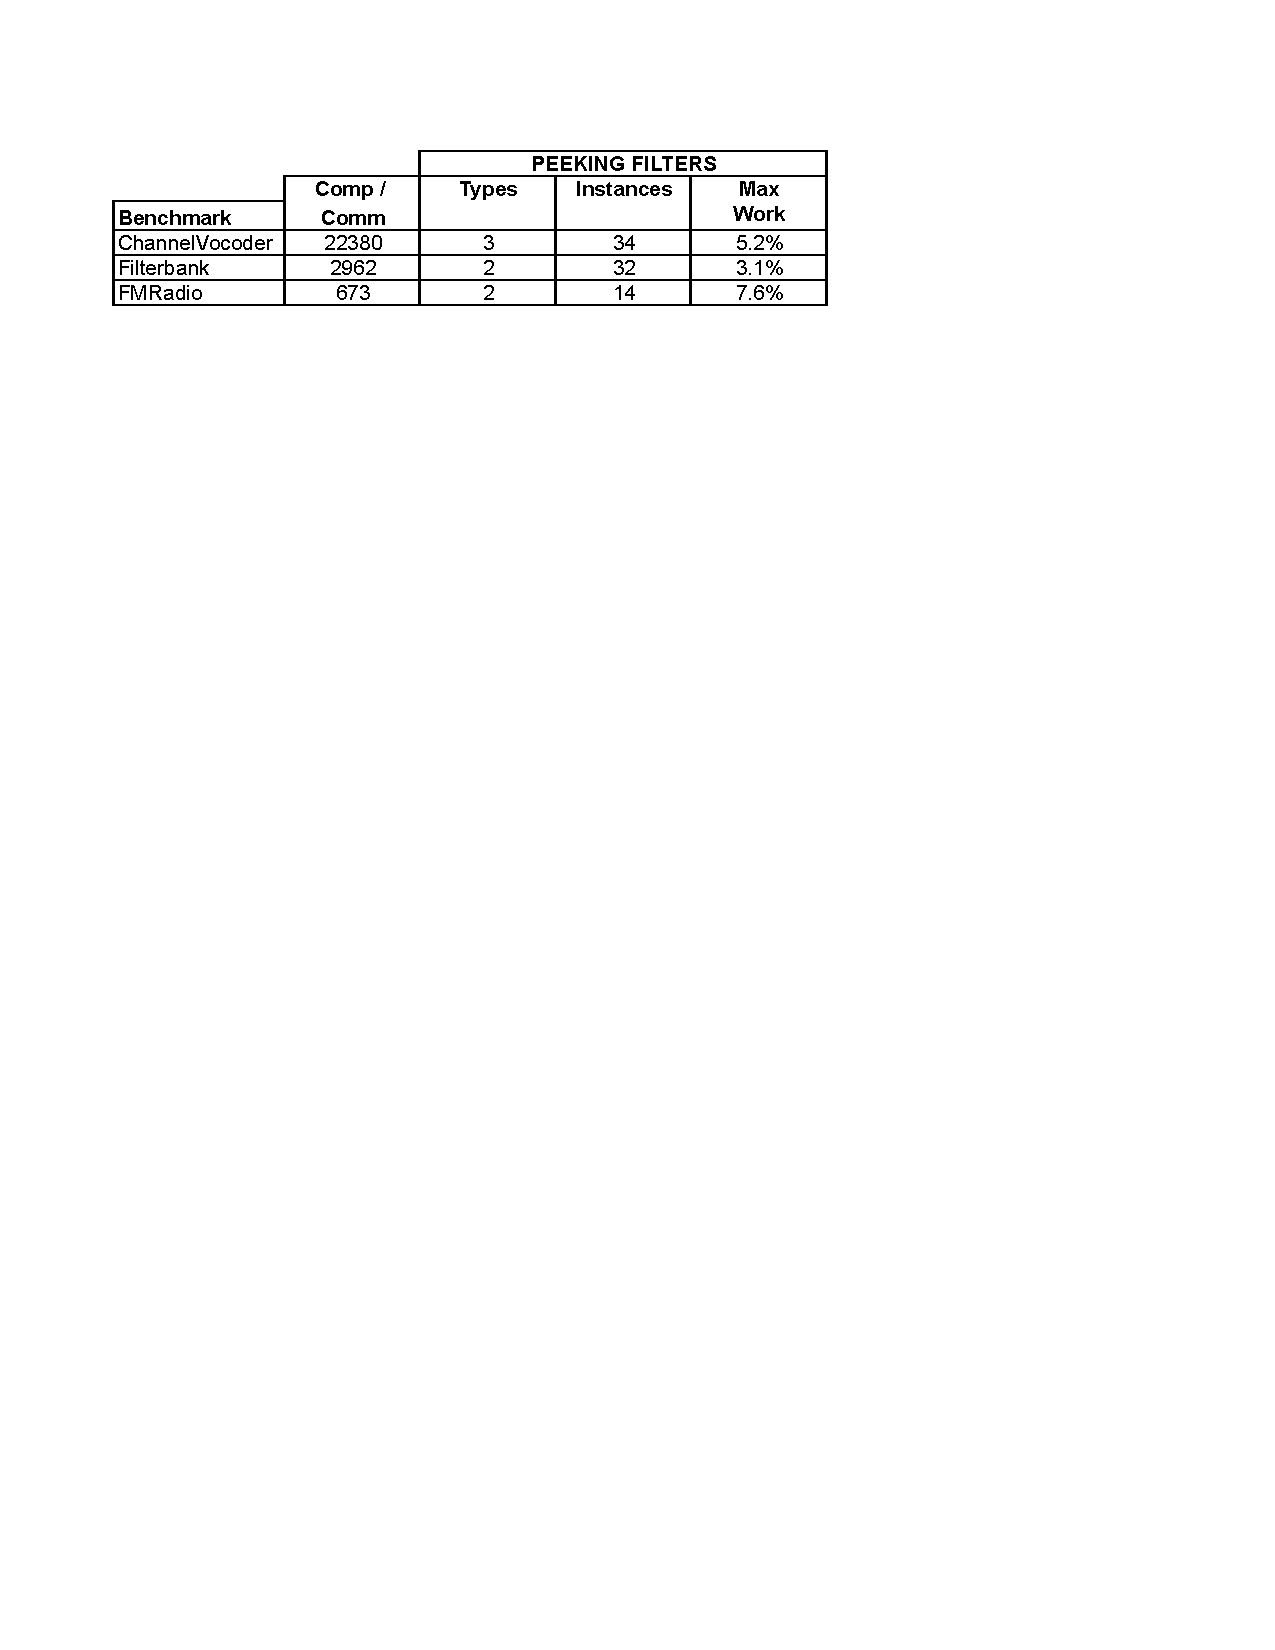
\includegraphics[width=3.3in]{figures/bench-char.pdf}}

\noindent ``Comp/Comm'' provides a static estimation of the
amount of computation to communication ratio by statically estimating the total
work of all the filters and dividing by the number items communicated
for the programmer-conceived graph's steady-state.  The remaining
statistics give the number of peeking filters types, number of peeking
filters instantiated at runtime, and a static estimation of the maximum
work in the single most loaded peeking filter.

We target 2 multicore architecture with different communication
mechanisms.  The Tilera Corporation's TILE64 Processor is a 64 core
system on a chip~\cite{tilera}.  Each core is an identical three-wide
VLIW. The code generated by the StreamIt
compiler for the TILE64 processor follows the remote store programming
(RSP) model~\cite{rsp10} in which each process has a private address
space, but each process can award remote processes write access to
their local memory. When a producer process has write access to a
consumer process's memory, the producer communicates directly with the
consumer via store instructions whose destination is an address in the
consumer's shared memory.  Communication is initiated by the producer,
and is fine-grained.  The consumer reads directly from it's local
memory (L2) when accessing input.

Our symmetric multiprocessor target is a 16-core architecture that is
comprised of four Intel Xeon E7350 multicore processors.  Each processor
is a 64-bit, quad-core with two dual-core dies.  Each die contains a 4
MB L2 cache shared across the two cores.  The front-side bus is clocked
at 1066 MHz.  We utilize the cache coherency mechanism of the
architecture for communication between cores. 

Through empirical experimentation on FMRadio, Filterbank, and
ChannelVocoder, we have settled on $T_{\mt{sharing}} =.10$ and
$T_{\mt{apply}} = 0.05$. These constants are the sweet stop for the two
architectures employed in the experimentation, being a good compromise
between buffer size and inter-core communication.

% \begin{figure*}[t]
% \centering
% \subfigure[]{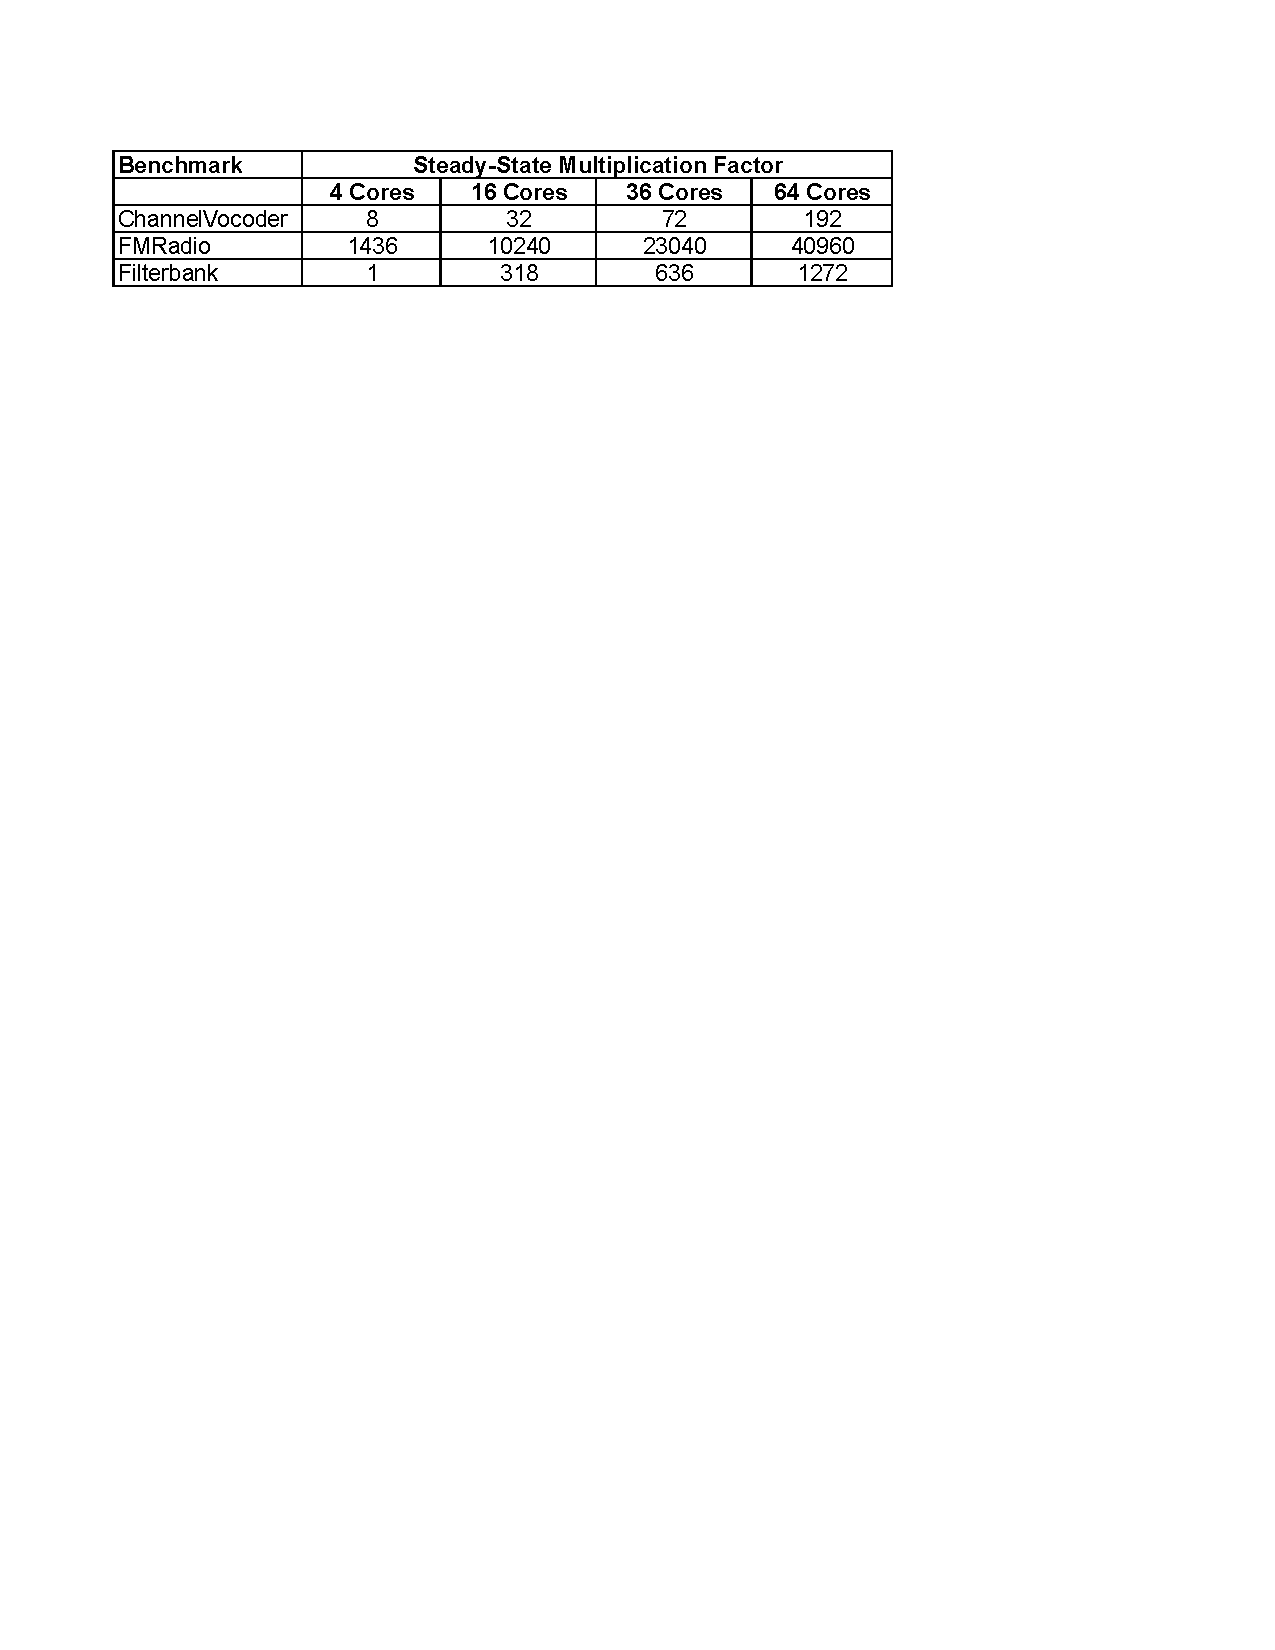
\includegraphics[width=3.7in]{figures/mult-table.pdf}} \\
% \subfigure[]{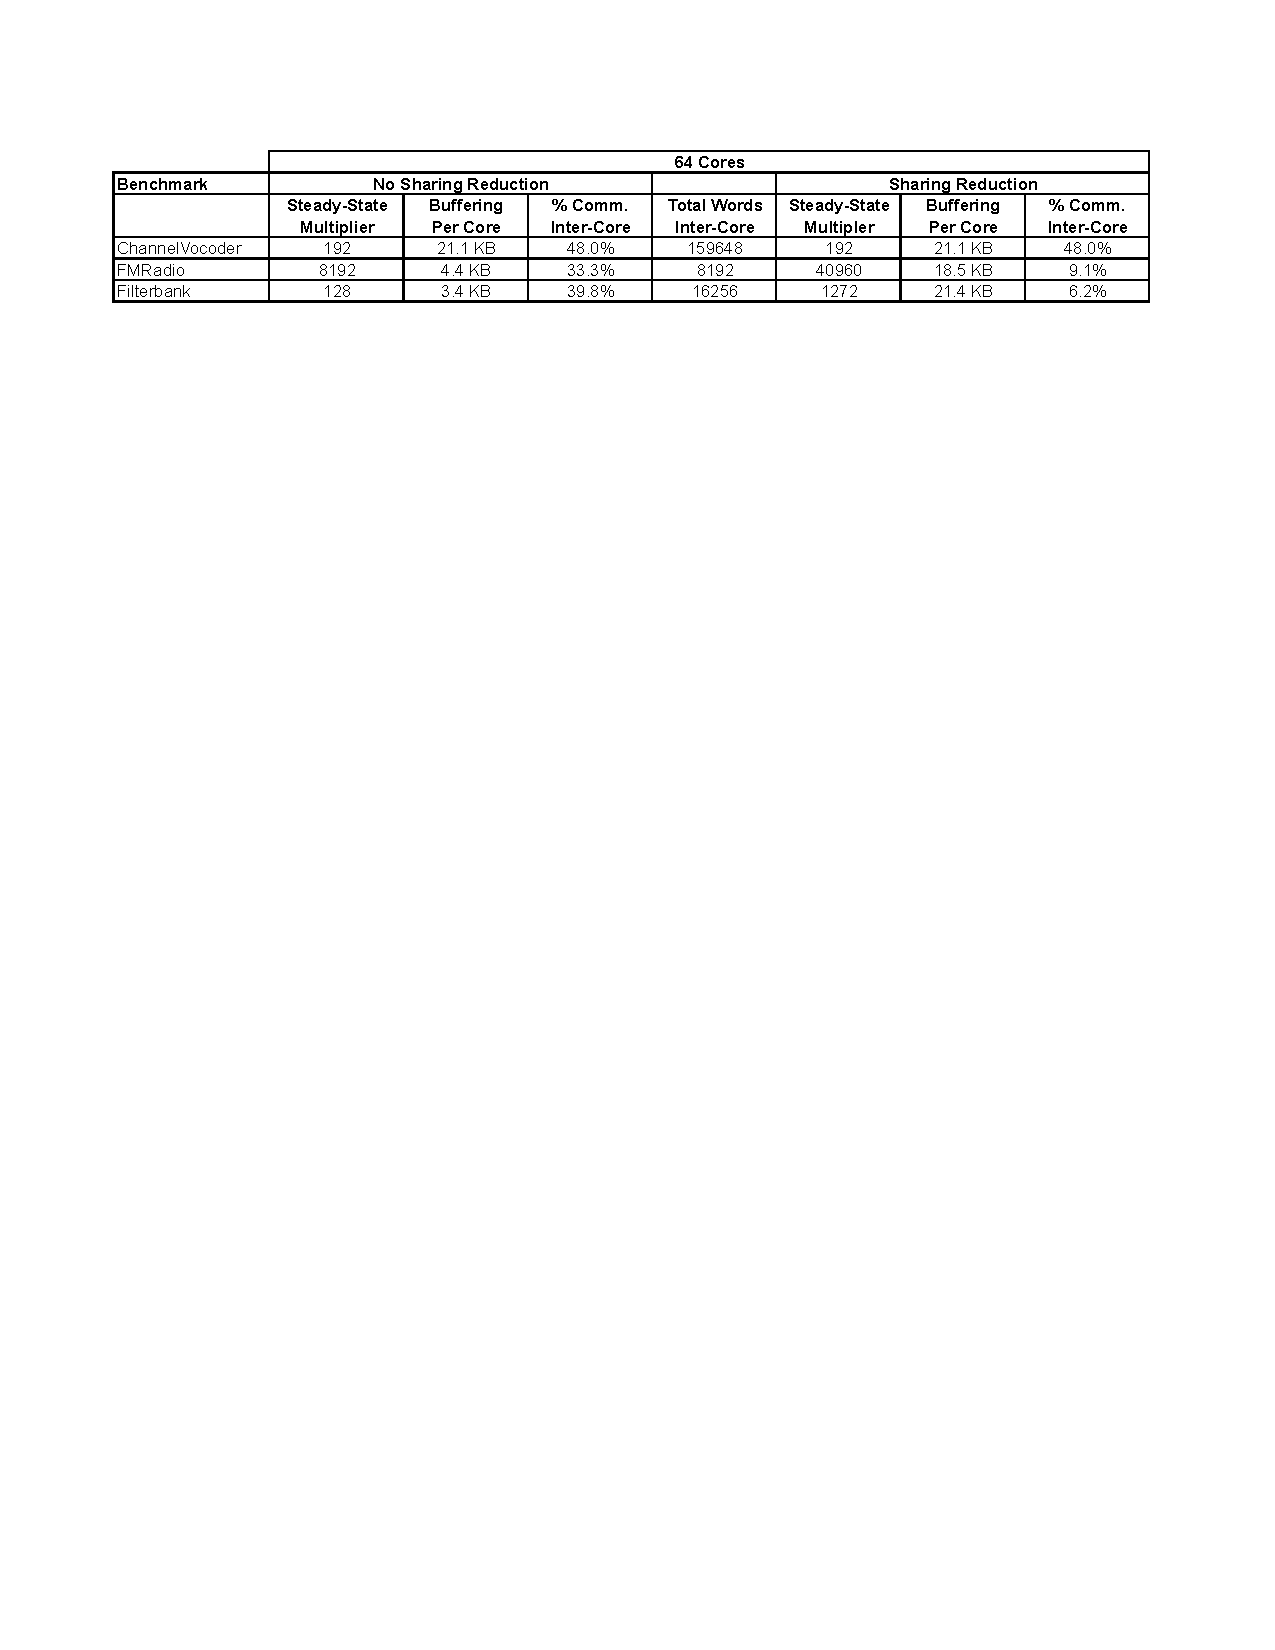
\includegraphics[width=6in]{figures/64-core-table.pdf}}
% \caption[Communication, multiplier and buffering statistics for
% benchmarks.]{
% Communication, multiplier and buffering characteristics for
% benchmarks: (a) gives the steady-state multipliers calculated for
% sharing reduction, (b) compares the steady-state with and without
% sharing reduction. 
% \label{fig:fission-table}}
% \end{figure*}

\begin{figure*}[t]
\centering
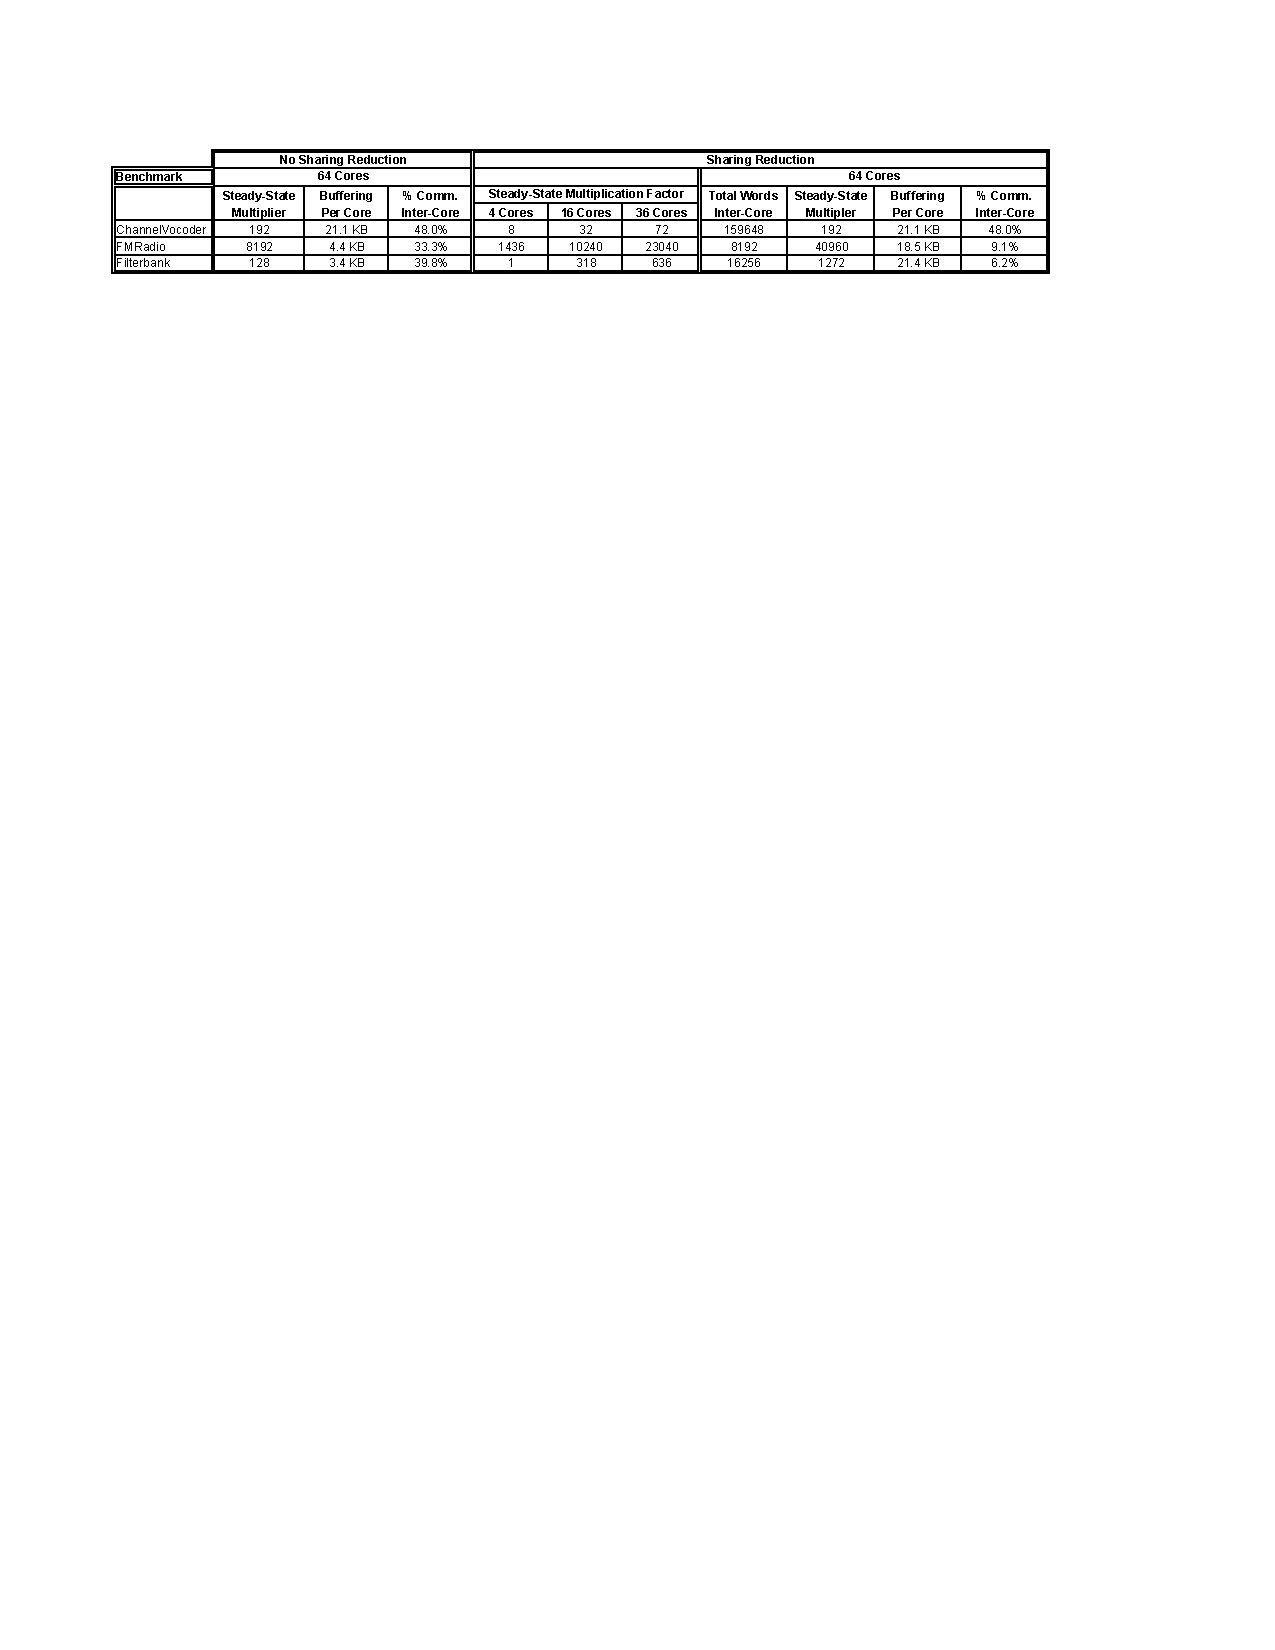
\includegraphics[width=6.1in]{figures/big-table.pdf}
\caption{\label{fig:big-table}  Steady-state multiplicity, buffering,
  and communication for fission with and without sharing reduction.}
\end{figure*}

% \begin{figure}[t]
% \centering
% 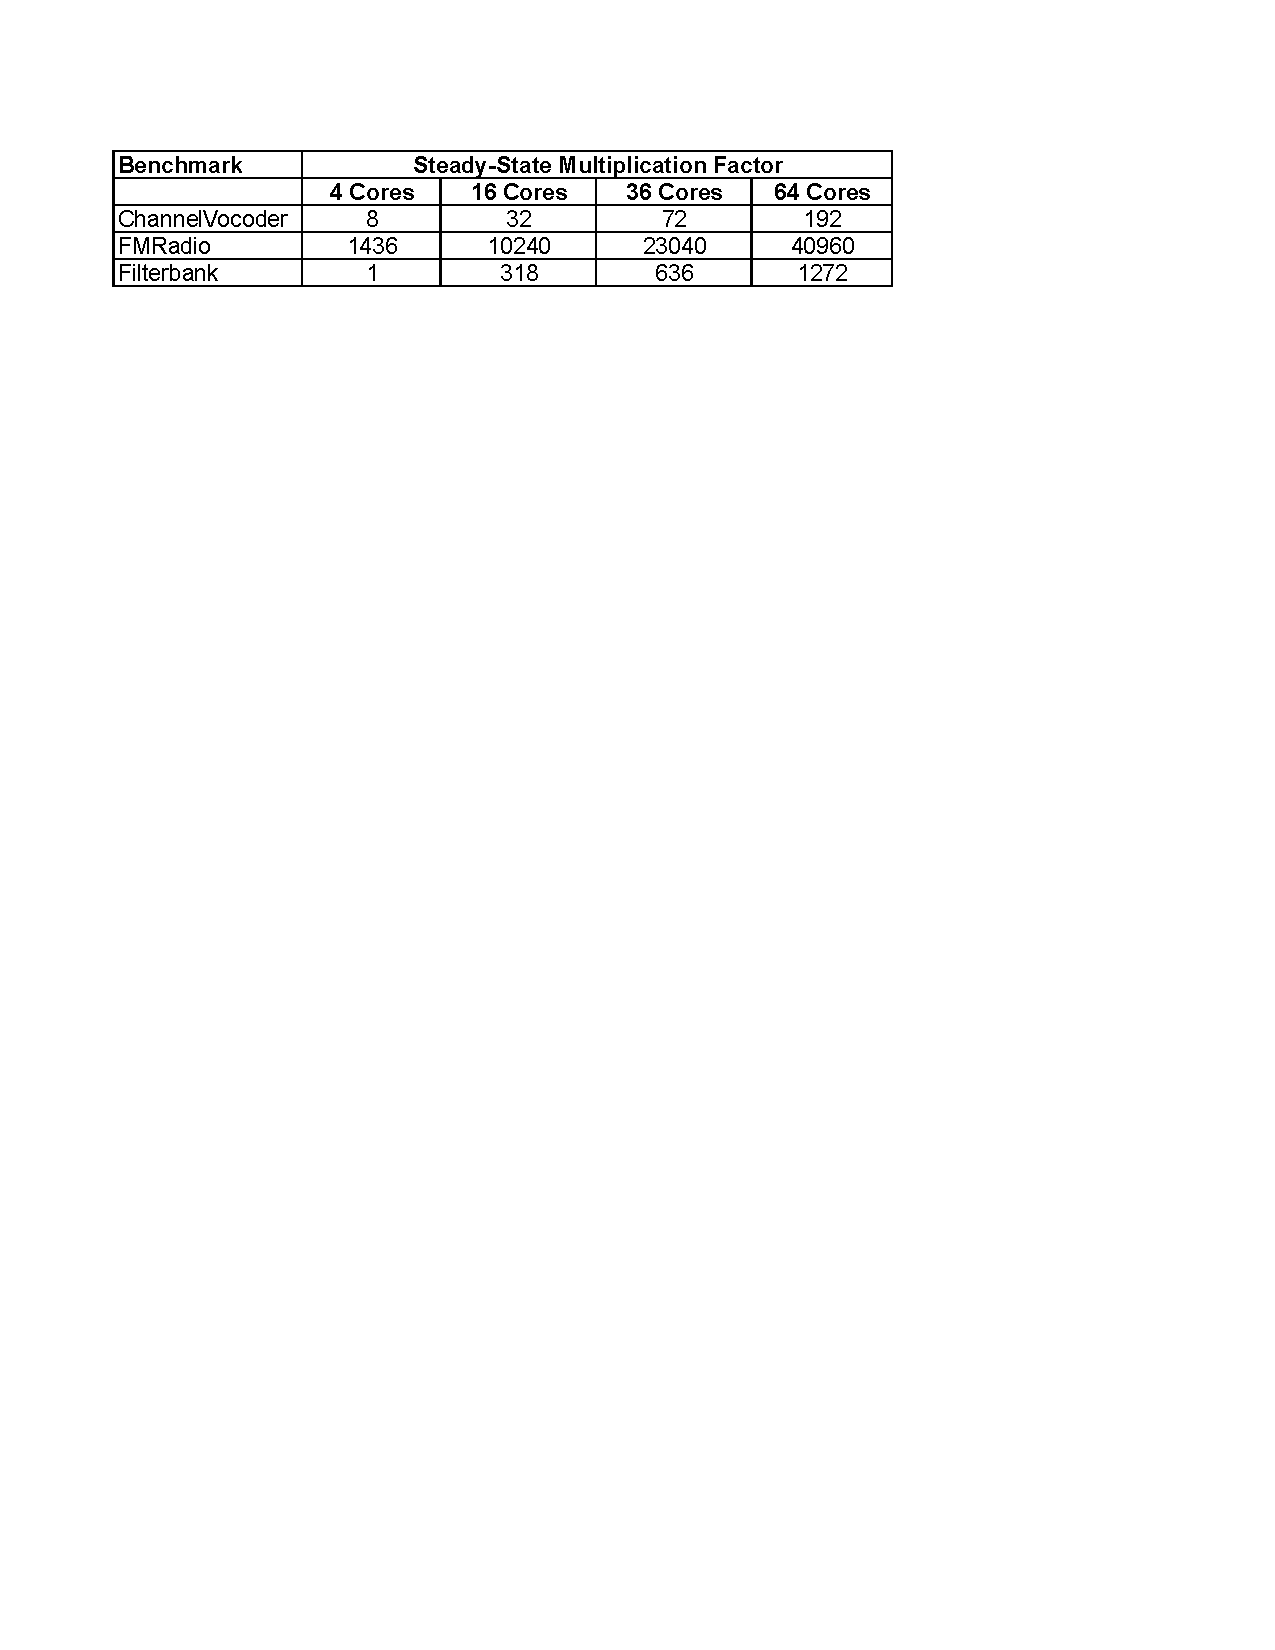
\includegraphics[width=3.3in]{figures/mult-table.pdf}
% \caption{\label{fig:mult-table}  The steady-state multipliers calculated for
% sharing reduction.}
% \end{figure}

% \begin{figure*}[t]
% \centering
% 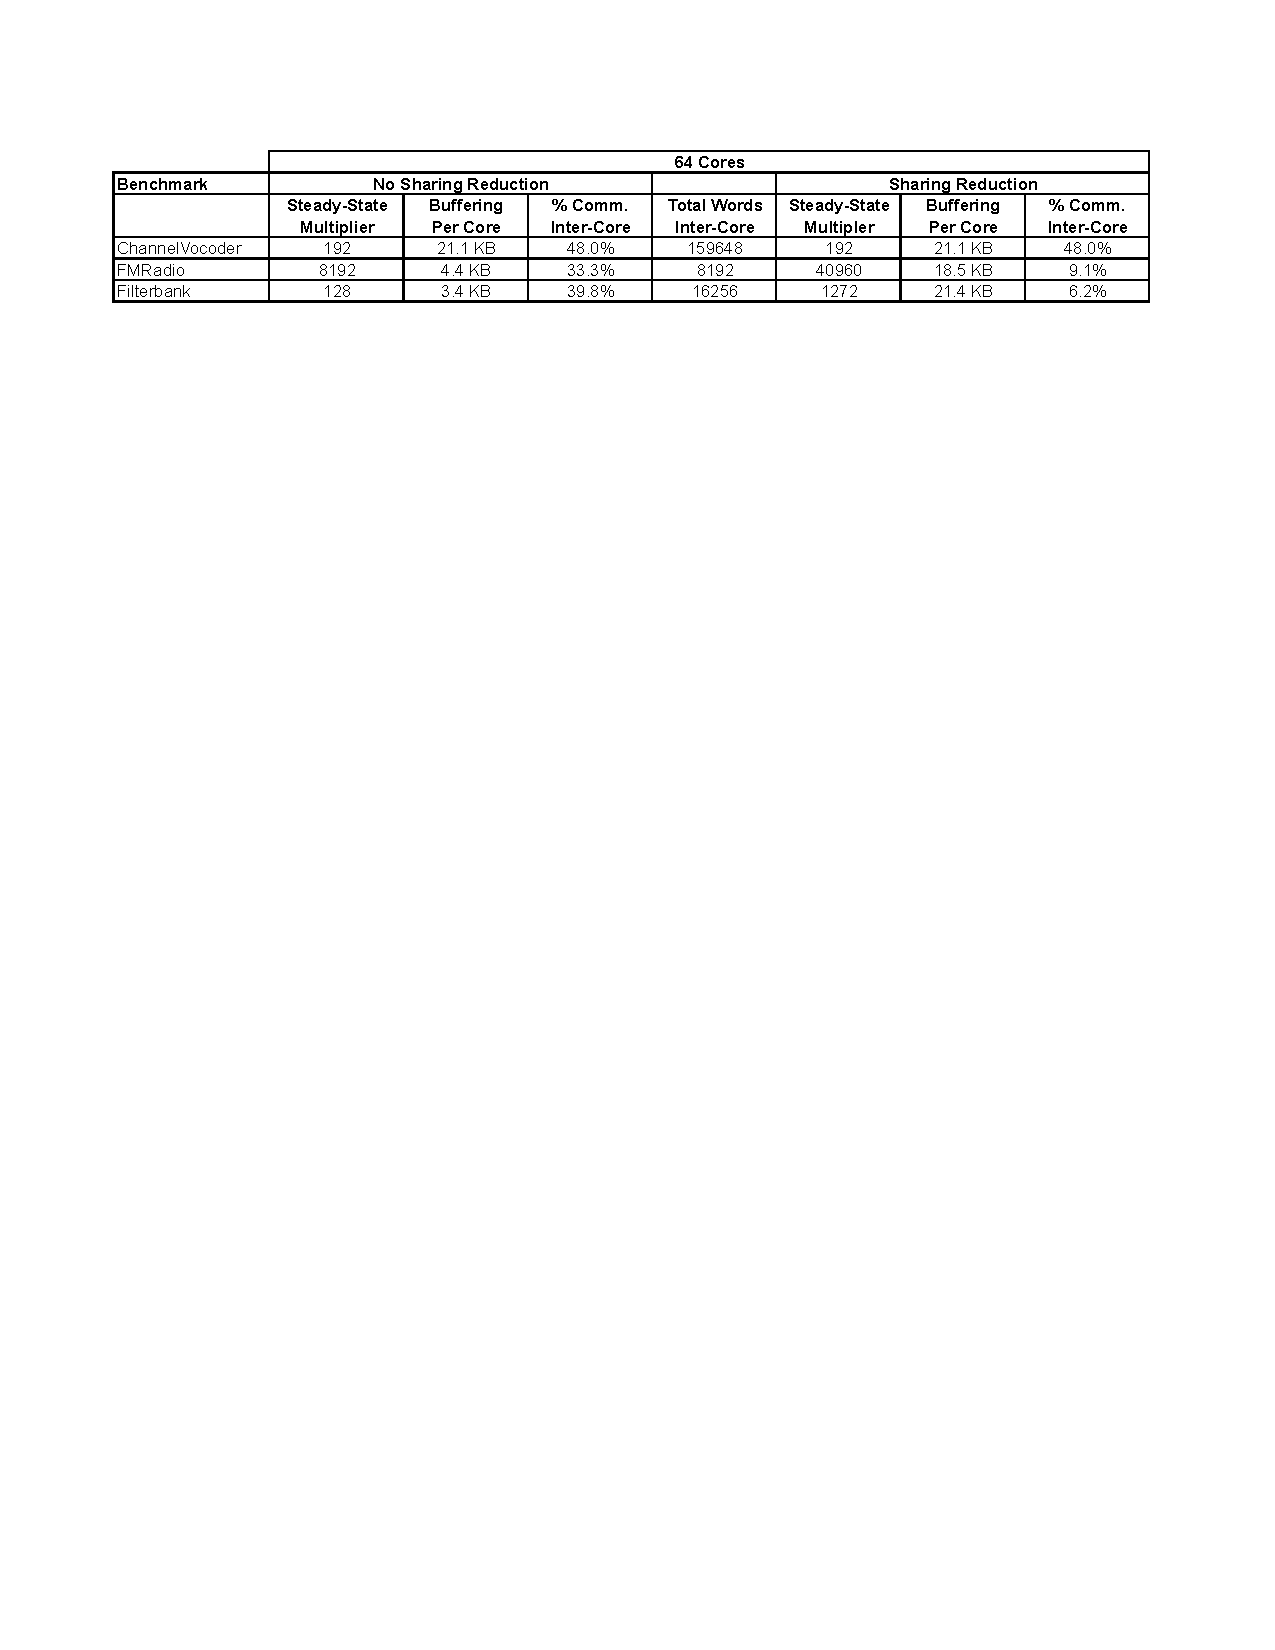
\includegraphics[width=6in]{figures/64-core-table.pdf}
% \caption{ Multiplier, buffering and communication for the steady-state with and without
% sharing reduction. 
% \label{fig:fission-table}}
% \end{figure*}

Figure~\ref{fig:big-table} compares the steady-state with and
without sharing reduction for a 64-core mapping, as well as gives the
constant $c$ calculated by sharing reduction for 4, 16, and 36.  The
factor is larger for FMRadio because one filter has $C(f) \gg o(S,
f)$.  The multiplication factor affects both latency and buffer sizes
adversely.  The application designer will have to decide if the
latency of these techniques can be borne given the application
criteria.  The total buffering requirement is increased when the
steady-state is increased.  However, since we are then fissing, the
buffer is divided amongst the fission products, and the {\it per-core}
buffering requirement is unaffected by the increase.  For example,
FMRadio, has a per-core 18 KB buffering requirement across all
configurations (4, 16, 36, and 64 cores).  This requirement fits in
the per-core L2 size of 64 KB for the Tile64.

 For ChannelVocoder,
sharing reduction has no effect because most of the peeking filters do
not satisfy $T_{\mt{apply}} = 0.05$ because of differing fission
factors between producers and consumers.  For the peeking filters that do,
the steady-state multiplier required for legal general fission for the
graph is enough to assure $T_{\mt{sharing}}$ is met.  Even though
sharing reduction has no effect for ChannelVocoder, general fission
avoids the 38\% of total items that were unnecessary duplicated by
DupDec.

For FMRadio and Filterbank, sharing reduction leads to significant
decreases in the percentage of total items communicated inter-core for
each steady-state.  The buffer requirement is increased an average of
5.2x for these benchmarks.  The total number of words communicated
inter-core during each steady-state is the same, with and without
sharing reduction.  However, the steady-state is greater in the
sharing reduction case, thus producing more outputs.

\begin{figure}[t]
\centering
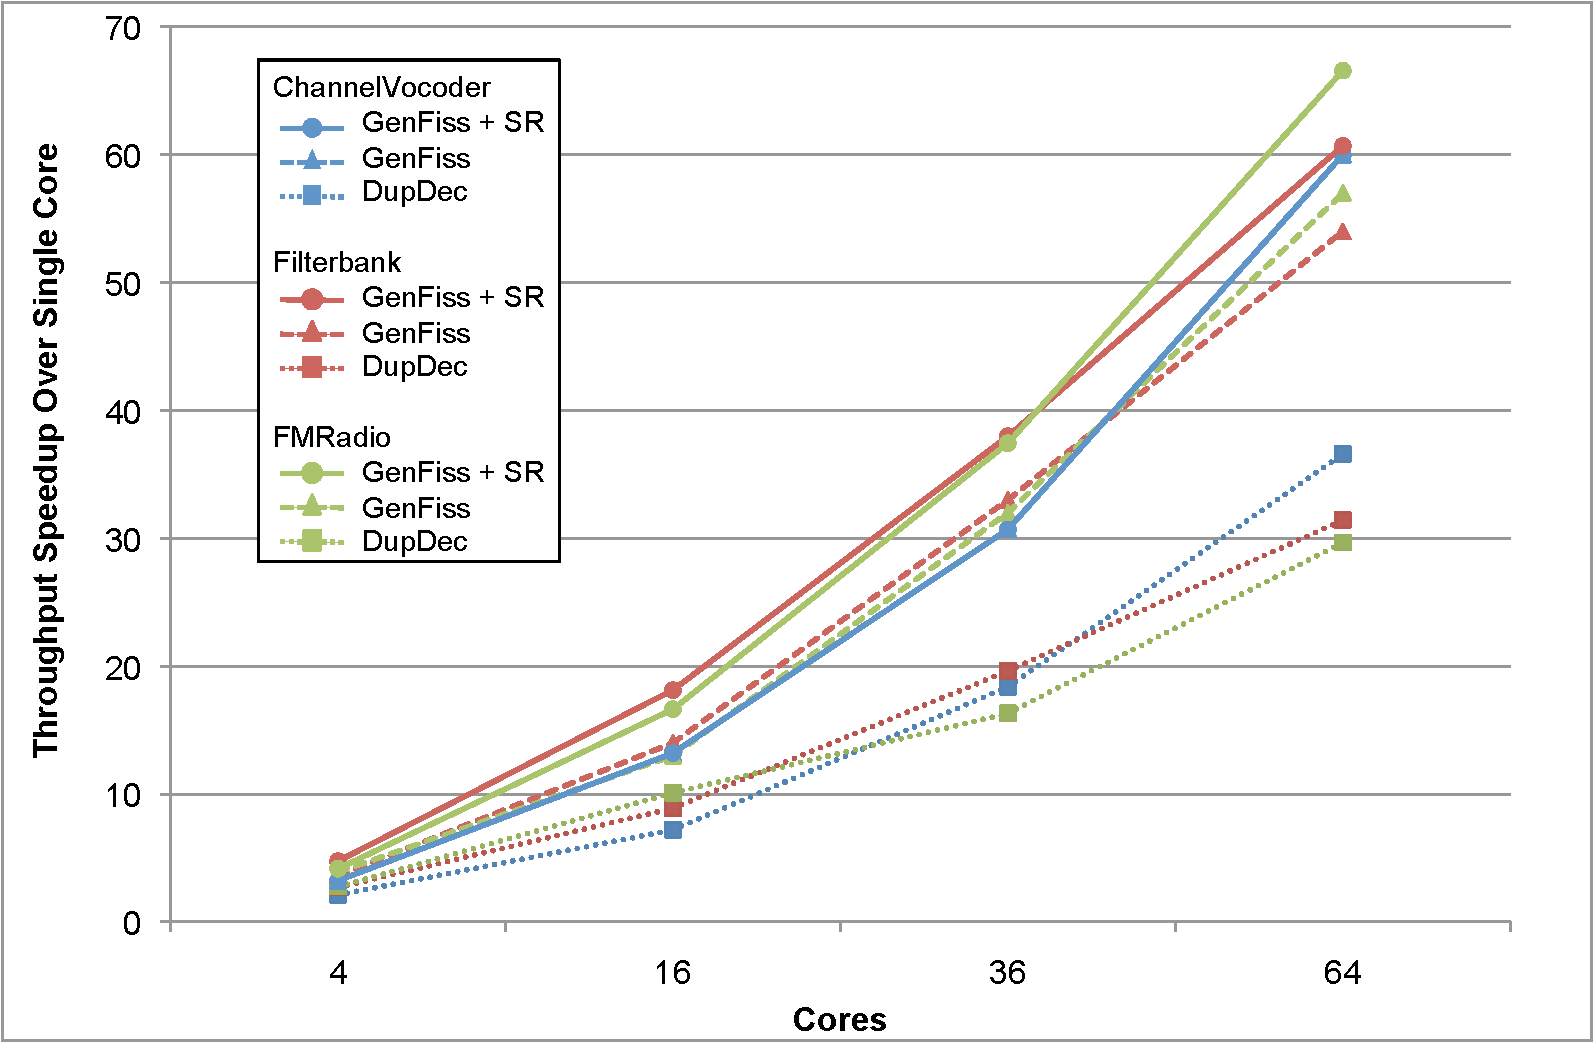
\includegraphics[width=3.3in]{figures/tilera-chart.pdf}
\caption[Comparing the fission techniques on the TILE64.]{
  Evaluation for DupDec versus general fission versus general fission with sharing reduction
  4, 16, 36, and 64 cores on the TILE64.  \label{fig:tilera-chart}}
\end{figure}

Figure~\ref{fig:tilera-chart} gives the performance results for the
Tilera TILE64 architecture.  We present results for DupDec, general
fission, and general fission with sharing reduction for 4, 16, 36, and
64 core configurations, with throughput normalized to single-core
throughput.  General fission with sharing reduction outperforms
DupDec by an average of 1.8x for the three benchmarks when targeting
64 cores. The average 64-core speedup over single core is 62.3x for the
general fission plus sharing reduction for these three benchmarks.

FMRadio experiences the most significant gain from general fission
plus sharing reduction over DupDec (67x versus 30x, respectively, for
64 cores).  FMRadio has the lowest computation to communication ratio
of the 3 benchmarks.  Furthermore, each filter of is fissed by the
number of cores targeted.  For 64 cores, each filter is fissed 64
ways.  DupDec must perform a global all-to-all communication involving
all 64 cores between each level of the graph!
 
ChannelVocoder achieves a 60x speedup for general fission over a
single core.  This is not perfectly linear because of the parallel
mapping; asymmetries exist between the extent of task parallelism and
the number of cores (see~\ref{mgordon-asplos06}).  The speedup over
DupDec (1.62x) is more modest because the width of many of the
fission applications is 3, so DupDec is duplicating input data to
groups of 3 filters.  Filterbank is similar, the width of fission is 4
for all filters when targeting 64 cores.

Sharing reduction is required to achieve scalable speedups for both
FMRadio and Filterbank.  For FMRadio, sharing reductions leads to a
17\% speedup increase for 64 cores.  This because sharing reduction
significantly reduces the number of remote write store instructions
required per output.  This affects FMRadio because of its low
computation to communication ratio.  Sharing reduction sees a 12\%
increase on Filterbank, as Filterbank has a larger computation to
communication ratio.

\begin{figure}[t]
\centering
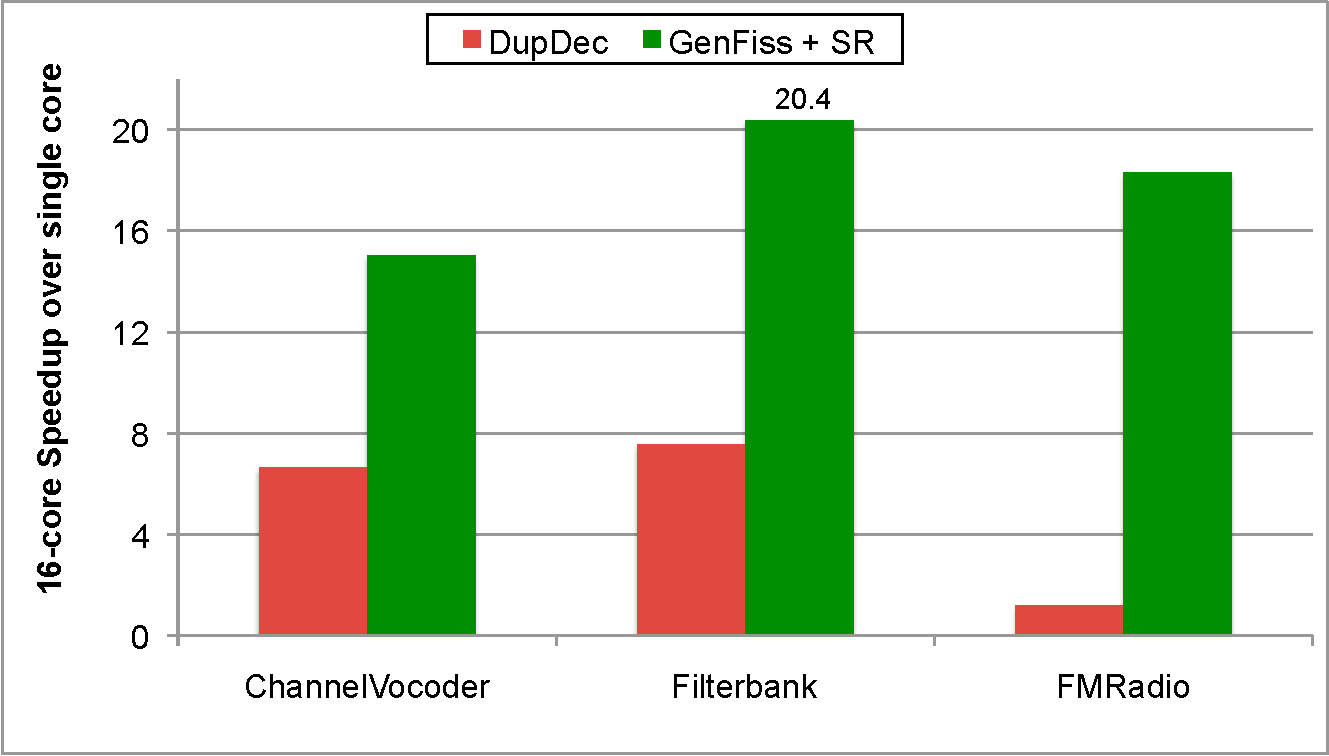
\includegraphics[width=3.3in]{figures/smp-chart.pdf}
\caption[Comparing the fission techniques on the 16-core SMP.]{
  Evaluation for DupDec versus general fission with sharing reduction
  for the 16-core SMP architecture.  \label{fig:smp-chart}}
\end{figure}

Our techniques enable scalable parallelization, with a mean speedup of
17x for our 3 benchmarks on the SMP.  Figure~\ref{fig:smp-chart} gives
the 16-core speedup comparison for DupDec versus general fission with
sharing reduction for our target SMP architecture.  The mean speedup
increase for general fission with sharing reduction over DupDec is
6.7x.  FMRadio again sees the largest speedup increase in the
comparison at 13.0x.  The reasons for this large speedup are similar
as given in the previous section.  However, the SMP communication
mechanism is not as efficient as the TILE64, thus general fission with
sharing reduction gives a greater speedup because reducing inter-core
communication has more impact.

%\section{Related Work}
\label{sec:related}

% BILL

%Signal~\cite{Signal}, 
%Lucid~\cite{Lucid77}, and
%Occam~\cite{Occam}, and Sisal \cite{sisal}.
%Parallel Haskell~\cite{ph}
In addition to StreamIt, there are a number of stream-oriented
languages drawing from domains such as functional, dataflow, CSP and
synchronous programming~\cite{survey97}.  The Brook language is
architecture-independent and focusses on data
parallelism~\cite{brook04}.  Stream kernels are required to be
stateless, though there is special support for reducing streams to a
single value.  Stream\-C/Ker\-nel\-C is lower level than Brook;
kernels written in KernelC are stiched together in StreamC and mapped
to the data-parallel Imagine processor~\cite{imagine03ieee}.  SPUR
adopts a similar decomposition between ``microcode'' stream kernels
and skeleton programs to expose data parallelism~\cite{spur05samos}.
Cg exploits pipeline parallelism and data parallelism, though the
programmer must write algorithms to exactly match the two pipeline
stages of a graphics processor~\cite{cg03}.  Compared to these
languages, StreamIt places more emphasis on exposing task and pipeline
parallelism (all the languages expose data parallelim).
%and on sliding window operations (filters that peek).  
By adopting the synchronous dataflow model of execution~\cite{lee87},
StreamIt focusses on well-structured programs that can be aggressively
optimized.  The implicit infinite loop around programs is also a key
StreamIt characteristic that enables the transformations in this
paper.  Spidle is also a recent stream language that was influenced by
StreamIt~\cite{spidle03}.
%and Lucid Synchrone~\cite{Lucid-Synchrone}.
%Synchronous languages which
%target embedded applications include Esterel~\cite{Esterel},
%Lustre~\cite{Lustre}, and Additional

Liao et al. map Brook to multicore processors by leveraging the affine
partitioning model~\cite{liao06brook}.  While affine partitioning is a
powerful model for parameterized loop-based programs, in StreamIt we
simplify the problem by fully resolving the program structure at
compile time.  This allows us to schedule a single steady state using
flexible, non-affine techniques (e.g., simulated annealing) and to
repeat the found schedule for an indefinite period at runtime.
Gummaraju and Rosenblum map stream programs to a general-purpose
hyperthreaded processor~\cite{gummaraju05micro}.  Such techniques
could be integrated with our spatial partitioning to optimize per-core
performance.  Gu et al. expose data and pipeline parallelism in a
Java-like language and use a compiler analysis to efficiently extract
coarse-grained filter boundaries~\cite{du03sc}.  Ottoni et al. also
extract decoupled threads from sequential code, using hardware-based
software pipelining to distribute the resulting threads across
cores~\cite{ottoni05decoupled}.  By embedding pipeline-parallel
filters in the programming model, we focus on the mapping step.

%%%%%%%%%%%%%%%%%%%%%%%%%%%%%%%%%%%%%%%%%%%%%%%%%%%%%%%%%%%%%%%%%%%%%

Previous work in scheduling computation graphs to parallel targets has
focused on partitioning and scheduling techniques that exploit task
and pipeline parallelism~\cite{SDFSched, SDFSched2,may87communicating,
DAGSched, pipeline-sdf}.  Application of loop-conscious
transformations to coarse-grained dataflow graphs has been
investigated.  Unrolling (or ``unfolding'' in this domain) is employed
for synchronous dataflow (SDF) graphs to reduce the initiation
interval but they do not evaluate mappings to actual
architectures~\cite{unfolding,unfolding2}. Software pipelining
techniques have been applied to SDF graphs onto various embedded and
DSP targets~\cite{bakshi99,chatha-02}, but has required programmer
knowledge of both the application and the architecture. To our
knowledge, none of these systems automatically exploit the combination
of task, data, and pipeline parallelism.  Furthermore, these systems
do not provide a robust end-to-end path for application
parallelization from a high-level, portable programming language.

%% Previous work on instruction-level software pipelining has focused
%% mostly on scheduling machine instructions in a loop via modulo
%% scheduling~\cite{rau81,lam-softpipe}.  The algorithms devised must
%% account for tight resource constraints and complex instruction
%% dependences. Our software-pipelining problem is much less constrained,
%% enabling us to employ a simple greedy heuristic.  

%% Furthermore, a traditional modulo scheduling algorithm is not needed
%% because we have an implicit loop barrier at the end of each
%% steady-state.  ILP compilers for clustered VLIW
%% architectures~\cite{Bulldog,Multiflow,lee98spacetime,qian02} must
%% partition instructions and assign them to clusters as part of the
%% instruction scheduling. Clustering is analogous to our application of
%% filter fusion in our software pipelining algorithm.

%\section{Conclusion}
\label{sec:conclusion}

In this paper, we describe the StreamIt compiler for the Raw
architecture.  The stream graph of a StreamIt program exposes the data
communication pattern to the compiler while the lack of global
synchronization frees the compiler to radically reoganize the program
for efficient execution on the underline architecture. The StreamIt
compiler demonstrates the power of this flexibility by totally
reoganizing large programs for better load balance. We were able to
map many of programs on to the Raw processor and obtain good
performance.

We introduce a collection of optimizations, vertical and horizontal
filter fusion, vertical and horizontal filter fission and filter
reordering transformations, that can be used to restructure stream
graphs.  We show that by applying these transformations we can map a
high-level stream program, written to reflect the composition of the
application, onto Raw and achieve good processor utilization and load
balance, leading to a factor of three speedup on two applications.

Unlike all previous streaming languages, the structured streams of
StreamIt makes it possible for us to approach the optimization and
parallelization problems in a very systermatic manner. It enables us
to define multiple optimizations -- targetting different constructs
and requirements -- and to compose them them in a hirearchical manner.

The ability to do global transformations across multiple filters, that
may have originated from very different parts of the application,
makes it possible for the compiler to find optimization opportunities
that may ellude even an experience programmer.  Such capabilities
enables the programmers to write protable streaming applications and
map them efficiently onto any given architecture. This has the
potential of creating a programming standard for emerging
communication exposed architectures.  The StreamIt compiler takes a
fist step towards this goal.



%\begin{small}
%\begin{singlespace}
%\bibliography{main}
%\bibliographystyle{abbrv}
%\end{singlespace}
%\end{small}

\end{document}
